% Preamble
\documentclass{beamer}
\usepackage[spanish]{babel}

% Packages
\usepackage{amsmath}
\usepackage[utf8]{inputenc}
\usepackage[T1]{fontenc}
\usepackage{graphicx}
\usepackage{algorithmicx}
\usepackage{algpseudocode}
\usepackage{caption}
\usepackage{courier}
\usepackage{amsmath}

\DeclareMathOperator{\atantwo}{atan2}


\captionsetup{justification=centering, font={scriptsize}, skip=0pt}

% Set bold vectors to satisfy requirements
\renewcommand\vec[1]{\ifstrequal{#1}{0}{\ensuremath{\mathbf{0}}}{\ensuremath{\boldsymbol{#1}}}}

\usetheme[compress]{Berlin}
\usecolortheme{wolverine}
\setbeamertemplate{page number in head/foot}[framenumber]
\setbeamercolor{institute in head/foot}{parent=palette primary}

\title[Dinámica Molecular Dirigida por Eventos]{Dinámica Molecular de Esferas Rígidas: Simulaciones Dirigidas por eventos}
\subtitle{72.25 - Simulación de Sistemas}
\author[Flores Lucey, Llanos]{Alejo Flores Lucey\inst{1} \and Nehuén Gabriel Llanos\inst{2}}
\institute[Instituto Tecnológico de Buenos Aires]
{
    \inst{1}
    \href{mailto:afloreslucey@itba.edu.ar}{afloreslucey@itba.edu.ar}\\
    Legajo 62622
    \and
    \inst{2}
    \href{mailto:nllanos@itba.edu.ar}{nllanos@itba.edu.ar}\\
    Legajo 62511
}
\date{2024 1C | Grupo Nº3}
\titlegraphic{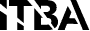
\includegraphics[height=0.5cm]{./itba}}

\makeatletter
\beamer@theme@subsectionfalse
\makeatother

\AtBeginSection[]{
    \begin{frame}
        \begin{beamercolorbox}[sep=8pt,center]{title}
            \usebeamerfont{title}\insertsection
        \end{beamercolorbox}
    \end{frame}
}

\begin{document}

    \begin{frame}
        \titlepage
    \end{frame}

    \section{Introducción}

        \begin{frame}{Introducción}
            \begin{itemize}
                \item \textbf{Objetivo:}
                \begin{itemize}
                    \item Simular un sistema de partículas en un espacio bidimensional.
                    \item Predecir propiedades de sistemas físicos a nivel de partículas.
                    \item Relacionar observables macroscópicos con dinámicas microscópicas.
                \end{itemize}
                \item \textbf{Modo de simulación:}
                \begin{itemize}
                    \item Simulación dirigida por eventos.
                    \item Se calculan los tiempos de colisión.
                    \item Se avanzan los estados hasta ese tiempo.
                \end{itemize}
            \end{itemize}
        \end{frame}

        \subsection{Sistema Real}

            \begin{frame}{Sistema Real}
                \begin{itemize}
                    \item Las partículas tienen un radio $r$ y una velocidad inicial $\vec{v}$.
                    \item Se estudia como colisionan entre sí y con las paredes del contenedor.
                \end{itemize}
                \begin{minipage}[t]{0.5\textwidth}
                    \begin{itemize}
                        \item \textbf{Aplicaciones:}
                        \begin{itemize}
                            \item Movimiento de moléculas de gas.
                            \item Dinámicas de reacciones químicas.
                            \item Desarrollo de videojuegos.
                        \end{itemize}
                    \end{itemize}
                \end{minipage}
                \hfill
                % HASTA ACA ESTA CAMBIADO
                \begin{minipage}[t]{0.45\textwidth}
                    \begin{figure}[H]
                        \centering
                        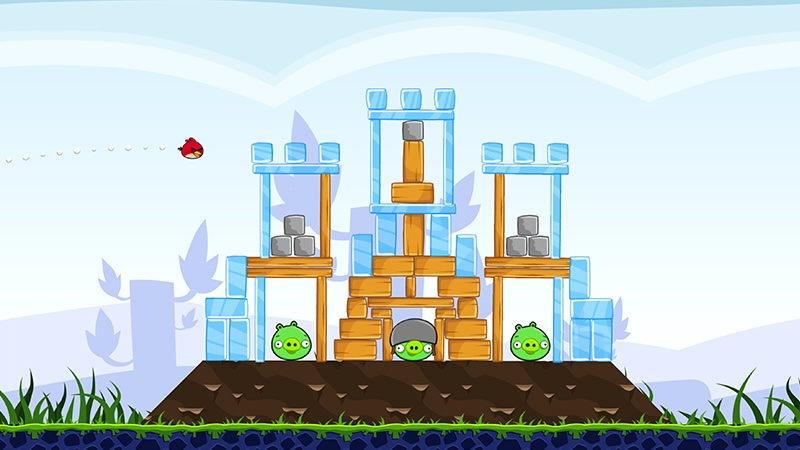
\includegraphics[width=\linewidth]{./angrybirds}
                        \label{fig:angry_birds}
                    \end{figure}
                \end{minipage}
            \end{frame}

        \subsection{Fundamentos}

            \begin{frame}{Fundamentos}
                \begin{itemize}
                    \item Las partículas son una 5-upla $(x, y, R, v_x, v_y)$
                    \item Las partículas se mueven en linea recta hasta que ocurre una colisión:
                        \begin{equation*}
                            \vec{x_i}(t+1) = \vec{x_i}(t) + \vec{v_i}(t) t_c\ ; \ t_c = \text{tiempo mínimo de colisión}
                        \end{equation*}
                    \item Se busca el tiempo en el que las partículas colisionan:
                        \begin{equation*}
                            \left( x_i - x_j \right) ^2 + \left( y_i - y_j \right) ^2 = \left( R_i + R_j \right) ^2
                        \end{equation*}
                    \item Las colisiones son elásticas y se conserva el impulso.
                \end{itemize}
            \end{frame}

    \section{Implementación}

        \subsection{Arquitectura}

            \begin{frame}{Diagrama UML}
                \begin{figure}[htbp]
                    \centering
                    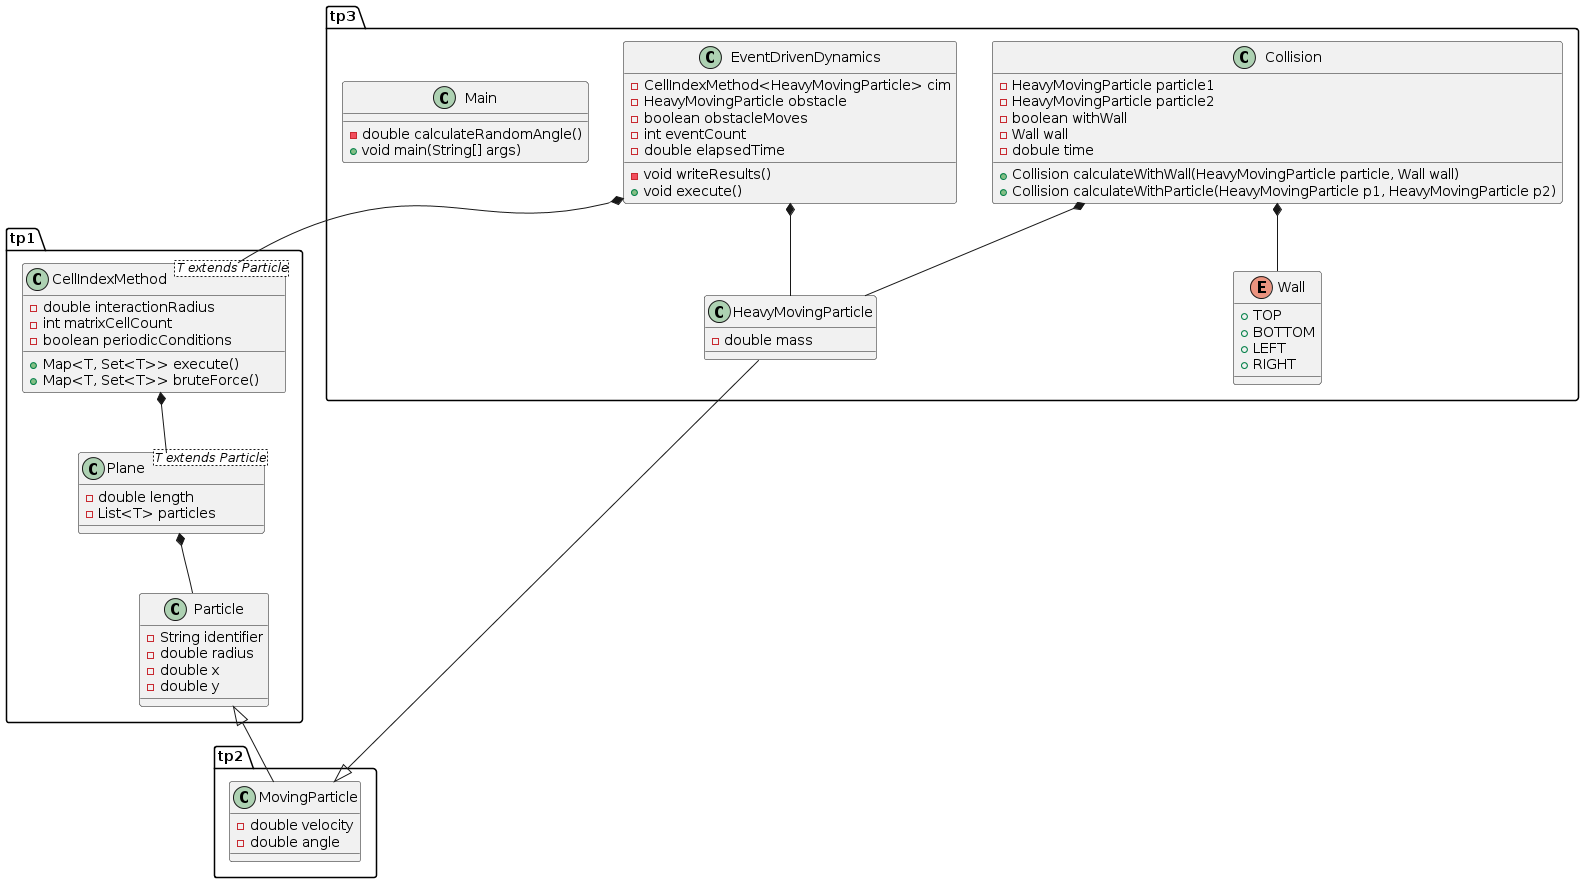
\includegraphics[width=\textwidth]{./architecture}
                    \label{fig:architecture}
                \end{figure}
            \end{frame}

        \subsection{Algoritmo}

            \begin{frame}{Pseudocódigo del algoritmo implementado}{}
                \begin{algorithmic}[1]
                    \ttfamily \scriptsize
                    \State Create output file
                    \State collisions $\gets$ new OrderedSet()
                    \ForAll{p $\in$ particles}
                        \State collisions $\gets$ \Call{CalculateCollisionsWithWalls}{p}
                        \ForAll{q $\in$ particles}
                            \State collisions $\gets$ \Call{CalculateCollisionsBetweenParticles}{p, q}
                        \EndFor
                    \EndFor
                    \While{$i < eventCount$}
                        \State first $\gets$ \Call{PopFirstCollision}{collisions}
                        \ForAll{p $\in$ particles}
                            \State \Call{Move}{p, first.time}
                        \EndFor
                        \State \Call{UpdateCollisionsTime}{first.time}
                        \State \Call{WriteOutput}{particles}
                        \State \Call{UpdateVelocities}{first.p1, first.p2}
                        \State \Call{CalculateNewCollisions}{first}
                        \State $i \gets i + 1$
                    \EndWhile
                \end{algorithmic}
            \end{frame}

    \section{Simulaciones}

        \subsection{Parámetros de entrada}

            \begin{frame}{Parámetros de entrada}
                \begin{itemize}
                    \item Parámetros de entrada fijos:
                    \begin{itemize}
                        \item Número de partículas ($N$): \alert{$300$}
                        \item Cantidad de eventos ($E$): \alert{$20.000$}
                        \item Longitud del plano ($L$): \alert{$0.1(m)$}
                        \item Radio de partículas ($r$): \alert{$0.001(m)$}
                        \item Radio del obstáculo ($R$): \alert{$0.005(m)$}
                        \item Masa de partículas ($m$): \alert{$1(kg)$}
                        \item Masa del obstáculo ($m$): \alert{$3(kg)$}
                    \end{itemize}
                    \item Parámetros de entrada variables:
                    \begin{itemize}
                        \item Módulo de la velocidad ($v$): \alert{$\{1, 3, 6, 10\}(m/s)$}
                    \end{itemize}
                \end{itemize}
            \end{frame}

        \subsection{Observables}

            \begin{frame}{Presión en paredes y obstáculo en función del tiempo ($P(t)$)}
                \begin{itemize}
                    \item Presión en paredes en función del tiempo:
                    \begin{equation*}
                        P_{Paredes}(t) = \frac{\sum \Delta V_{n\ (Paredes)}}{\Delta t \cdot L \cdot 4}
                    \end{equation*}
                    \begin{equation*}
                        V_{n\ (Paredes\ Sup.\ y\ Inf.)} = \left| v \cdot \sin(\alpha) \cdot 2 \right|
                    \end{equation*}
                    \begin{equation*}
                        V_{n\ (Paredes\ Izq.\ y\ Der.)} = \left| v \cdot \cos(\alpha) \cdot 2 \right|
                    \end{equation*}
                    \item Presión en el obstáculo en función del tiempo:
                    \begin{equation*}
                        P_{Obst\acute{a}culo}(t) = \frac{\sum \vec{V_{n\ (Obst\acute{a}culo)}}}{\Delta t \cdot 2\pi \cdot R}
                    \end{equation*}
                    \begin{equation*}
                              \vec{V_{n\ (Obst\acute{a}culo)}} = \left| {v \cdot \cos \left( \atantwo \left(\frac{L}{2} - y, \frac{L}{2} - x \right) \right) \cdot 2} \right|
                    \end{equation*}
                \end{itemize}
            \end{frame}

            \begin{frame}{Tiempo en el que el nro. de choques alcanza el 20\% de $N$ }
                \begin{itemize}
                    \item Se realizan diez (10) corridas.
                    \item Se estudia el tiempo en el que el 20\% de las partículas colisionan por primera vez con el obstáculo.
                    \begin{equation*}
                        t_{\text{prom}} = \frac{\sum_{i=1}^{10} t_i}{10} \ ,\ t_i\text{: tiempo en corrida }i
                    \end{equation*}
                    \begin{equation*}
                              \sigma = \sqrt{\frac{1}{9} \sum_{i=1}^{10} (t_i - t_{\text{prom}})^2}
                    \end{equation*}
                \end{itemize}
            \end{frame}

            \begin{frame}{Número de choques por unidad de tiempo}
                \begin{itemize}
                    \item Se calcula la pendiente de la curva mediante el método de regresión lineal simple
                    \begin{equation*}
                        \begin{split}
                            m_k(\iota) = \frac{\iota \sum_{i=1}^\iota x_i y_i - \sum_{i=1}^\iota x_i \sum_{i=1}^\iota y_i }{\iota \sum_{i=1}^\iota x_i^2 - \left(\sum_{i=1}^\iota x_i \right)^2}
                            \ , 1 \leq k \leq 10
                            \\ \iota = \text{cantidad de choques en el intervalo de tiempo}
                        \end{split}
                    \end{equation*}
                    \item Se promedian los valores obtenidos de cada una de las diez (10) corridas y se calcula su error asociado:
                    \begin{equation*}
                            m_{prom} = \frac{1}{10} \sum_{i=1}^{10} m_i
                        \text{ ; }
                            \sigma = \sqrt{\frac{1}{9} \sum_{i=1}^{10} (m_i - m_{\text{prom}})^2}
                    \end{equation*}
                \end{itemize}
            \end{frame}

            \begin{frame}{Desplazamiento cuadrático medio ($DCM$)}
                \begin{itemize}
                    \item Se realiza para cuatro (4) velocidades y diez (10) corridas cada una.
                    \item Se divide el intervalo de tiempo en cien (100) $\Delta t's$.
                    \item Se obtiene el desplazamiento cuadrático medio para cada $\Delta t$:
                    \begin{equation*}
                        DCM_{\Delta t} = \frac{\sum_{i=1}^{10} \left( x_{t_i} - x_0 \right)^2 + \left( y_{t_i} - y_0 \right)^2}{10}
                    \end{equation*}

                \end{itemize}
            \end{frame}

            \begin{frame}{Coeficiente de difusión ($D$)}
                \begin{itemize}
                    \item Se obtiene la pendiente de la curva de $DCM$ en función del tiempo mediante el método
                    de regresión lineal simple para cada velocidad.
                    \begin{equation*}
                        m_v = \frac{100 \sum_{i=1}^{100} x_i y_i - \sum_{i=1}^{100} x_i \sum_{i=1}^{100} y_i }{100 \sum_{i=1}^{100} x_i^2
                        - \left(\sum_{i=1}^{100} x_i \right)^2},\ v \in \{1, 3, 6, 10\}
                    \end{equation*}
                    \item Se obtiene el coeficiente de difusión:
                    \begin{equation*}
                        D_v = \frac{m_v}{4},\ v \in \{1, 3, 6, 10\}
                    \end{equation*}
                \end{itemize}
            \end{frame}


    \section{Resultados}

        \subsection{Parámetro de orden $v_a$}

            \begin{frame}{Parámetro de orden $v_a$}{Animación}
                \begin{minipage}[t]{0.60\textwidth}
                    \begin{figure}[H!]
                        \includegraphics[height=.65\textheight]{./animation-n300-eta0p6-frame}
                        \caption*{Véase la animación completa en \url{https://youtu.be/q8ep24AgTzU}.}
                        \label{fig:va_1}
                    \end{figure}
                \end{minipage}
                \hfill
                \begin{minipage}[t]{0.30\textwidth}
                    \begin{block}{Datos del sistema}
                        \begin{itemize}
                            \item $N=300$
                            \item $L=5$
                            \item $\eta=0.6$
                        \end{itemize}
                    \end{block}
                \end{minipage}
            \end{frame}

            \begin{frame}{Parámetro de orden $v_a$}{Animación}
                \begin{minipage}[t]{0.60\textwidth}
                    \begin{figure}[H!]
                        \includegraphics[height=.65\textheight]{./animation-n300-eta2p4-frame}
                        \caption*{Véase la animación completa en \url{https://youtu.be/aZ9eOtlXgQw}.}
                        \label{fig:va_2}
                    \end{figure}
                \end{minipage}
                \hfill
                \begin{minipage}[t]{0.30\textwidth}
                    \begin{block}{Datos del sistema}
                        \begin{itemize}
                            \item $N=300$
                            \item $L=5$
                            \item $\eta=2.4$
                        \end{itemize}
                    \end{block}
                \end{minipage}
            \end{frame}

            \begin{frame}{Parámetro de orden $v_a$}{Animación}
                \begin{minipage}[t]{0.60\textwidth}
                    \begin{figure}[H!]
                        \includegraphics[height=.65\textheight]{./animation-n300-eta5p2-frame}
                        \caption*{Véase la animación completa en \url{https://youtu.be/QkXskl_8CGs}.}
                        \label{fig:va_3}
                    \end{figure}
                \end{minipage}
                \hfill
                \begin{minipage}[t]{0.30\textwidth}
                    \begin{block}{Datos del sistema}
                        \begin{itemize}
                            \item $N=300$
                            \item $L=5$
                            \item $\eta=5.2$
                        \end{itemize}
                    \end{block}
                \end{minipage}
            \end{frame}

            \begin{frame}{Parámetro de orden $v_a$}{$v_a$ en función del tiempo}
                    \begin{figure}[H!]
                        \includegraphics[width=0.9\textwidth]{./va_vs_time-n300}
                        \label{fig:va_4}
                    \end{figure}
                    \begin{beamercolorbox}[sep=5pt,center]{block body}
                        \begin{minipage}[t]{0.45\textwidth}
                            \centering
                            \small{$N=300$}
                        \end{minipage}
                        \hfill
                        \begin{minipage}[t]{0.45\textwidth}
                            \centering
                            \small{$L=5$}
                        \end{minipage}
                    \end{beamercolorbox}
            \end{frame}

            \begin{frame}{Parámetro de orden $v_a$}{$v_a$ en función del ruido ($\eta$)}
                \begin{figure}[H!]
                    \includegraphics[width=0.9\textwidth]{./va_vs_eta}
                    \label{fig:va_5}
                \end{figure}
                \begin{beamercolorbox}[sep=5pt,center]{block body}
                    \small{$L=5$}
                \end{beamercolorbox}
            \end{frame}

        \subsection{Tiempo en el que el nro. de visitas alcanza el 20\% de $N$}

            \begin{frame}{Tiempo en el que el nro. de visitas alcanza el 20\% de $N$}{Animación}
                \begin{minipage}[t]{0.60\textwidth}
                    \begin{figure}[H!]
                        \includegraphics[height=.65\textheight]{animation_visits_pbc-n300-eta0p6-frame}
                        \caption*{Véase la animación completa en \url{https://youtu.be/MGHMlVLz0Ys}.}
                        \label{fig:pbc_1}
                    \end{figure}
                \end{minipage}
                \hfill
                \begin{minipage}[t]{0.30\textwidth}
                    \begin{block}{Datos del sistema}
                        \begin{itemize}
                            \item $N=300$
                            \item $L=5$
                            \item $\eta=0.6$
                        \end{itemize}
                    \end{block}
                \end{minipage}
            \end{frame}

            \begin{frame}{Tiempo en el que el nro. de visitas alcanza el 20\% de $N$}{Cantidad total de visitas en función del tiempo}
                \begin{figure}[H!]
                    \includegraphics[width=0.9\textwidth]{./visits_vs_time_pbc-n300-eta0p6}
                    \label{fig:pbc_2}
                \end{figure}
                \begin{beamercolorbox}[sep=5pt,center]{block body}
                    \begin{minipage}[t]{0.3\textwidth}
                        \centering
                        \small{$N=300$}
                    \end{minipage}
                    \hfill
                    \begin{minipage}[t]{0.3\textwidth}
                        \centering
                        \small{$L=5$}
                    \end{minipage}
                    \hfill
                    \begin{minipage}[t]{0.3\textwidth}
                        \centering
                        \small{$\eta=0.6$}
                    \end{minipage}
                \end{beamercolorbox}
            \end{frame}

            \begin{frame}{Tiempo en el que el nro. de visitas alcanza el 20\% de $N$}{Observable en función del ruido ($\eta$)}
                \begin{figure}[H!]
                    \includegraphics[width=0.9\textwidth]{./threshold_vs_eta-pbc}
                    \label{fig:pbc_3}
                \end{figure}
                \begin{beamercolorbox}[sep=5pt,center]{block body}
                    \small{$L=5$}
                \end{beamercolorbox}
            \end{frame}

        \subsection{Nro. de visitas por unidad de tiempo}

            \begin{frame}{Nro. de visitas por unidad de tiempo}{Animación}
                \begin{minipage}[t]{0.60\textwidth}
                    \begin{figure}[H!]
                        \includegraphics[height=.65\textheight]{./animation_visits_obc-n300-eta0p6-frame}
                        \caption*{Véase la animación completa en \url{https://youtu.be/ZcCPUwjMHBc}.}
                        \label{fig:obc_1}
                    \end{figure}
                \end{minipage}
                \hfill
                \begin{minipage}[t]{0.30\textwidth}
                    \begin{block}{Datos del sistema}
                        \begin{itemize}
                            \item $N=300$
                            \item $L=5$
                            \item $\eta=0.6$
                        \end{itemize}
                    \end{block}
                \end{minipage}
            \end{frame}

            \begin{frame}{Nro. de visitas por unidad de tiempo}{Cantidad total de visitas en función del tiempo}
                \begin{figure}[H!]
                    \includegraphics[width=0.9\textwidth]{./visits_vs_time_obc-n300}
                    \label{fig:obc_2}
                \end{figure}
                \begin{beamercolorbox}[sep=5pt,center]{block body}
                    \begin{minipage}[t]{0.45\textwidth}
                        \centering
                        \small{$N=300$}
                    \end{minipage}
                    \hfill
                    \begin{minipage}[t]{0.45\textwidth}
                        \centering
                        \small{$L=5$}
                    \end{minipage}
                \end{beamercolorbox}
            \end{frame}

            \begin{frame}{Nro. de visitas por unidad de tiempo}{Observable en función del ruido ($\eta$)}
                \begin{figure}[H!]
                    \includegraphics[width=0.9\textwidth]{./slope_vs_eta-obc}
                    \label{fig:obc_3}
                \end{figure}
                \begin{beamercolorbox}[sep=5pt,center]{block body}
                    \small{$L=5$}
                \end{beamercolorbox}
            \end{frame}

    \section{Conclusiones}

        \begin{frame}{Conclusiones}
            \begin{itemize}
                \item Se observó que a medida que aumenta la cantidad de partículas, la polarización tiende a ser
                levemente mayor.
                \item En las visitas PBC se puede notar que:
                \begin{itemize}
                    \item a medida que el ruido se incrementa, el tiempo en el que el número de visitas alcanza un
                    porcentaje de $N$ también aumenta.
                    \item para valores de baja cantidad de partículas y/o alto ruido, no se alcanza ese umbral.
                \end{itemize}
                \item En las visitas OBC se puede contemplar que:
                \begin{itemize}
                    \item la cantidad de visitas por unidad de tiempo disminuye a medida que el ruido aumenta, sin importar el $N$.
                    \item para valores altos de $\eta$, la cantidad de partículas que visitan las zonas es acotada.
                \end{itemize}
            \end{itemize}
        \end{frame}

\end{document}
